%% abtex2-modelo-trabalho-academico.tex, v-1.9.6 laurocesar
%% Copyright 2012-2016 by abnTeX2 group at http://www.abntex.net.br/ 
%%
%% This work may be distributed and/or modified under the
%% conditions of the LaTeX Project Public License, either version 1.3
%% of this license or (at your option) any later version.
%% The latest version of this license is in
%%   http://www.latex-project.org/lppl.txt
%% and version 1.3 or later is part of all distributions of LaTeX
%% version 2005/12/01 or later.
%%
%% This work has the L PPL maintenance status `maintained'.
%% 
%% The Current Maintainer of this work is the abnTeX2 team, led
%% by Lauro César Araujo. Further information are available on 
%% http://www.abntex.net.br/
%%
%% This work consists of the files abntex2-modelo-trabalho-academico.tex,
%% abntex2-modelo-include-comandos and abntex2-modelo-references.bib
% ------------------------------------------------------------------------
% ------------------------------------------------------------------------
% abnTeX2: Modelo de Trabalho Academico (tese de doutorado, dissertacao de
% mestrado e trabalhos monograficos em geral) em conformidade com 
% ABNT NBR 14724:2011: Informacao e documentacao - Trabalhos academicos -
% Apresentacao
% ------------------------------------------------------------------------
% ------------------------------------------------------------------------
% Personalização para o modelo Udesc 2024 9. ed. revisada e modificada
% Manual_13_05_2024_17175220258266_12510.pdf acesso em: 13/08/2024
% Autor: Felipe Joel Zimann (felipezimann@hotmail.com)
% Data: 02/12/2020 v1.0
% Data: 13/02/2021 v1.0.1 alterado tamanho numeração da página para 10pt
% Data: 13/08/2024 v1.0.2 alterado para citação (Autor, Ano) ao invés de (AUTOR, Ano) conforme ABNT NBR 10520:2023
% ------------------------------------------------------------------------
% ------------------------------------------------------------------------

\documentclass[
	12pt,					% tamanho da fonte
	openright,				% capítulos começam em pág ímpar (insere página vazia caso preciso)
	oneside,				% para impressão em recto e verso (twoside). Oposto a (oneside)
	a4paper,				% tamanho do papel. 
	chapter=TITLE,			% títulos de capítulos convertidos em letras maiúsculas
	section=TITLE,			% títulos de seções convertidos em letras maiúsculas
	sumario=abnt-6027-2012,
	english,				% idioma adicional para hifenização
	brazil,					% o último idioma é o principal do documento
	fleqn,					% equações alinhadas a esquerda (UDESC/CCT)+
	]{abntex2}

% ----------------------------------------------------------
% Pacotes básicos 
% ----------------------------------------------------------
\usepackage{amsmath}							% Pacote matemático
% \usepackage{amssymb}							% Pacote matemático
% \usepackage{amsfonts}							% Pacote matemático
%\usepackage{lmodern}							% Usa a fonte Latin Modern		
% \usepackage{mathptmx} 							% Usa a fonte Times New Roman	 (UDESC/CCT)
% \usepackage[T1]{fontenc}						% Selecao de codigos de fonte.
% \usepackage[utf8]{inputenc}						% Codificacao do documento (conversão automática dos acentos)
% \usepackage{lastpage}							% Usado pela Ficha catalográfica
\usepackage{indentfirst}						% Indenta o primeiro parágrafo de cada seção.
% \usepackage[dvipsnames,table]{xcolor}			% Controle das cores
% \usepackage{graphicx}							% Inclusão de gráficos
\usepackage{microtype} 							% para melhorias de justificação
% \usepackage{lipsum}								% para geração de dummy text
\usepackage[brazilian,hyperpageref]{backref}	% Paginas com as citações na bibl
\usepackage[alf,abnt-emphasize=bf,abnt-full-initials=yes]{abntex2cite}					% Citações padrão ABNT
%\usepackage[num]{abntex2cite}					% Citações padrão ABNT numérica
% \usepackage{adjustbox}							% Pacote de ajuste de boxes
% \usepackage{subcaption}							% Inclusão de Subfiguras e sublegendas		
% \usepackage{enumitem}							% Personalização de listas
\usepackage{siunitx}							% Grandezas e unidades
% \usepackage[section]{placeins}					% Manter as figuras delimitadas na respectiva seção com a opção [section]
\usepackage{multirow}							% Multi colunas nas tabelas
\usepackage{array,tabularx} 					% Pacotes de tabelas
\usepackage{booktabs}							% Pacote de tabela profissonal
% \usepackage{rotating}							% Rotacionar figuras e tabelas
% \usepackage{xfrac}								% Fazer frações n/d em linha
% \usepackage{bm}									% Negrito em modo matemático
% \usepackage{xstring}							% Manipulação de strings
\usepackage{pgfplots}							% Pacote de Gráficos
\usepackage{tikz}								% Pacote de Figuras
\usepackage[american, cuteinductors,smartlabels, fulldiode, siunitx, americanvoltages, oldvoltagedirection, smartlabels]{circuitikz}						% Pacote de circuitos elétricos
\usepackage{chemformula}						% Pacote para fórmulas químicas
\usepackage{chngcntr}							% Pacte usado para deixar numeração de equações sequencial (UDESC/CCT)
\counterwithout{equation}{chapter}
% fonte: https://latex.org/forum/viewtopic.php?t=15392

% Comando para deixar numeração das equações contínua (1), (2), (3)... ao invés de organizar por capítulos (1.1)(1.2)... (2.1)(2.2)
%\renewcommand{\theequation}{\arabic{equation}}

%\numberwithin{equation}{section}


% Cabecalho cabeçalho somente com numeração de página 10pt
\makepagestyle{PagNumReduzida}
\makeevenhead{PagNumReduzida}{\ABNTEXfontereduzida\thepage}{}{}
\makeoddhead{PagNumReduzida}{}{}{\ABNTEXfontereduzida\thepage}
%fonte: https://github.com/abntex/abntex2/wiki/HowToCustomizarCabecalhoRodape
%fonte: Manual memoir seção 7.3 pg. 111 pdf http://linorg.usp.br/CTAN/macros/latex/contrib/memoir/memman.pdf 

% Personalização das opções das listas
\setlist[itemize]{leftmargin=\parindent}

% Citação online --- MODIFICAR ---
\newcommand{\citeshort}[1]{\citeauthoronline{#1}~(\citeyear{#1})}

\newcommand{\me}[1]{Elaborado pelo autor (#1).}

% Configuração do pgfplots
\pgfplotsset{compat=newest} %compat=1.14
\pgfplotsset{plot coordinates/math parser=false} 
\newlength\figureheight 
\newlength\figurewidth 

% % Libraries do TiKz
% \usetikzlibrary{quotes,angles,arrows}
% \usetikzlibrary{through,calc,math}
% \usetikzlibrary{graphs,backgrounds,fit}
% \usetikzlibrary{shapes,positioning,patterns,shadows}
% \usetikzlibrary{decorations.pathreplacing}
% \usetikzlibrary{shapes.geometric}
% \usetikzlibrary{arrows.meta}
% \usetikzlibrary{external}

% %\tikzexternalize[]
% %\tikzexternalenable
% %\tikzexternalize
% %\tikzexternaldisable
% %\tikzset{external/force remake}
% %\tikzexternalize[shell escape=-enable-write18]

% % Configurações do CircuiTiKz
% \ctikzset{bipoles/thickness=1}
% %\ctikzset{bipoles/length=1.2cm}
% \ctikzset{monopoles/ground/width/.initial=.2}
% \ctikzset{bipoles/resistor/height=0.25}
% \ctikzset{bipoles/resistor/width=0.6}
% \ctikzset{bipoles/capacitor/height=0.5}
% \ctikzset{bipoles/capacitor/width=0.15}
% \ctikzset{bipoles/generic/height=0.25}
% \ctikzset{bipoles/generic/width=0.6}
% %\ctikzset{bipoles/capacitor polar/length=0.5}
% %\ctikzset{bipoles/diode/height=.375}
% %\ctikzset{bipoles/diode/width=.3}
% %\ctikzset{tripoles/thyristor/height=.8}
% %\ctikzset{tripoles/thyristor/width=1}
% \ctikzset{bipoles/vsourcesin/height=.5}
% \ctikzset{bipoles/vsourcesin/width=.5}
% \ctikzset{bipoles/cvsourceam/height=.6}
% \ctikzset{bipoles/cvsourceam/width=.6}
% %\ctikzset{tripoles/european controlled voltage source/width=.4}

% \tikzstyle{every node}=[font=\footnotesize]
% \tikzstyle{every path}=[line width=0.25pt,line cap=round,line join=round]
%\tikzstyle{every path}=[line cap=round,line join=round]


% Definição de cores MATLAB
\definecolor{matlab_blue}{rgb}	{         0,    0.4470,    0.7410}
\definecolor{matlab_orange}{rgb}{    0.8500,    0.3250,    0.0980}
\definecolor{matlab_yellow}{rgb}{    0.9290,    0.6940,    0.1250}
\definecolor{matlab_violet}{rgb}{    0.4940,    0.1840,    0.5560}
\definecolor{matlab_green}{rgb}	{	 0.4660,    0.6740,    0.1880}
\definecolor{matlab_lblue}{rgb}	{    0.3010,    0.7450,    0.9330}
\definecolor{matlab_red}{rgb}	{    0.6350,    0.0780,    0.1840}

% Personalização das legendas
\usepackage[format = plain, %hang
			justification = centering,
			labelsep = endash,
			singlelinecheck = false,
			skip = 6pt,
			listformat = simple]{caption}	

% Personalização das unidades
\sisetup{output-decimal-marker = {,}}
\sisetup{exponent-product = \cdot}
\sisetup{tight-spacing=true}
\sisetup{group-digits = false}

% Personalizações de tipo de colunas de tabelas
\newcolumntype{L}[1]{>{\raggedright\let\newline\\\arraybackslash\hspace{0pt}}m{#1}}
\newcolumntype{C}[1]{>{\centering\let\newline\\\arraybackslash\hspace{0pt}}m{#1}}
\newcolumntype{R}[1]{>{\raggedleft\let\newline\\\arraybackslash\hspace{0pt}}m{#1}}

% Personalizações de cores da UDESC
\definecolor{CapaAmareloUDESC}{RGB}{243,186,83}		% Especializacao
\definecolor{CapaVerdeUDESC}{RGB}{0,112,52}			% Mestrado
\definecolor{CapaVermelhoUDESC}{RGB}{171,35,21}		% Doutorado
\definecolor{CapaAzulUDESC}{RGB}{38,54,118} 		% Pós-Doutorado

% CONFIGURAÇÕES DE PACOTES
% Configurações do pacote backref
% Usado sem a opção hyperpageref de backref
\renewcommand{\backrefpagesname}{Citado na(s) página(s):~}
% Texto padrão antes do número das páginas
\renewcommand{\backref}{}
% Define os textos da citação
\renewcommand*{\backrefalt}[4]{
	\ifcase #1 %
	Nenhuma citação no texto.%
	\or
	Citado na página #2.%
	\else
	Citado #1 vezes nas páginas #2.%
	\fi}%

% alterando o aspecto da cor azul
%\definecolor{blue}{RGB}{41,5,195}

% informações do PDF
\makeatletter
\hypersetup{
	%pagebackref=true,
	pdftitle={\@title}, 
	pdfauthor={\@author},
	pdfsubject={\imprimirpreambulo},
	pdfcreator={LaTeX with abnTeX2},
	pdfkeywords={abnt}{latex}{abntex}{abntex2}{trabalho academico}, 
	colorlinks=true,       		% false: boxed links; true: colored links
	linkcolor=black,          	% color of internal links
	citecolor=black,        	% color of links to bibliography
	filecolor=black,      		% color of file links
	urlcolor=black,
	bookmarksdepth=4
}
\makeatother


\makeatletter
\newcommand{\includetikz}[1]{%
	\tikzsetnextfilename{#1}%
	\input{#1.tex}%
}
\makeatother


% ---
% Possibilita criação de Quadros e Lista de quadros.
% Ver https://github.com/abntex/abntex2/issues/176
%
\newcommand{\quadroname}{Quadro}
\newcommand{\listofquadrosname}{Lista de quadros}

\newfloat[chapter]{quadro}{loq}{\quadroname}
\newlistof{listofquadros}{loq}{\listofquadrosname}
\newlistentry{quadro}{loq}{0}

% configurações para atender às regras da ABNT
\setfloatadjustment{quadro}{\centering}
\counterwithout{quadro}{chapter}
\renewcommand{\cftquadroname}{\quadroname\space} 
\renewcommand*{\cftquadroaftersnum}{\hfill--\hfill}

\setfloatlocations{quadro}{hbtp} % Ver https://github.com/abntex/abntex2/issues/176
% ---


% Espaçamento depois do título
\setlength{\afterchapskip}{0.7\baselineskip}
% O tamanho do parágrafo é dado por:
\setlength{\parindent}{1.25cm}
% Controle do espaçamento entre um parágrafo e outro:
\setlength{\parskip}{0.0cm}  % tente também \onelineskip
%\SingleSpacing % Espaçamento simples 
\OnehalfSpacing % Espaçamento 1,5 (UDESC/CCT)
%\DoubleSpacing	% Espaçamento duplo

% ---
% Margens - NBR 14724/2011 - 5.1 Formato
% ---
\setlrmarginsandblock{3cm}{2cm}{*}
\setulmarginsandblock{3cm}{2cm}{*}
\checkandfixthelayout[fixed]
% ---


% To use externalize consider
%https://tex.stackexchange.com/questions/182783/tikzexternalize-not-compatible-with-miktex-2-9-abntex2-package
%Lauro Cesar digged into the problem until he came with a solution for me to test. And it Works!
%
%According to this link:
%
%The package calc changed the commands \setcounter and friends to be fragile. So you have to make them robust. The example below uses etoolbox with \robustify:
%
\usepackage{etoolbox}
\robustify\setcounter
\robustify\addtocounter
\robustify\setlength
\robustify\addtolength


%% How to silence memoir class warning against the use of caption package?
%% https://tex.stackexchange.com/questions/391993/how-to-silence-memoir-class-warning-against-the-use-of-caption-package
%\usepackage{silence}
%\WarningFilter*{memoir}{You are using the caption package with the memoir class}
%\WarningFilter*{Class memoir Warning}{You are using the caption package with the memoir class}

% --------------------------------------------------------
% INICIO DAS CUSTOMIZACOES PARA A UDESC
% --------------------------------------------------------

% --------------------------------------------------------
% Fontes padroes de part, chapter, section, subsection e subsubsection
% --------------------------------------------------------
% --- Chapter ---
\renewcommand{\ABNTEXchapterfont}{\fontseries{b}} %\bfseries
\renewcommand{\ABNTEXchapterfontsize}{\normalsize}
% --- Part ---
\renewcommand{\ABNTEXpartfont}{\ABNTEXchapterfont}
\renewcommand{\ABNTEXpartfontsize}{\LARGE}
% --- Section ---
\renewcommand{\ABNTEXsectionfont}{\normalfont}
\renewcommand{\ABNTEXsectionfontsize}{\normalsize}
% --- SubSection ---
\renewcommand{\ABNTEXsubsectionfont}{\fontseries{b}} %\bfseries
\renewcommand{\ABNTEXsubsectionfontsize}{\normalsize}
% --- SubSubSection ---
\renewcommand{\ABNTEXsubsubsectionfont}{\itshape}
\renewcommand{\ABNTEXsubsubsectionfontsize}{\normalsize}

\renewcommand{\ABNTEXsubsubsubsectionfont}{\normalfont}
\renewcommand{\ABNTEXsubsubsubsectionfontsize}{\normalsize}
% ---

% --------------------------------------------------------
% Fontes das entradas do sumario
% --------------------------------------------------------

\renewcommand{\cftpartfont}{\ABNTEXpartfont\selectfont}
\renewcommand{\cftpartpagefont}{\normalsize\selectfont}

\renewcommand{\cftchapterfont}{\ABNTEXchapterfont\selectfont}
\renewcommand{\cftchapterpagefont}{\normalsize\selectfont}

\renewcommand{\cftsectionfont}{\ABNTEXsectionfont\selectfont}
\renewcommand{\cftsectionpagefont}{\normalsize\selectfont}

\renewcommand{\cftsubsectionfont}{\ABNTEXsubsectionfont\selectfont}
\renewcommand{\cftsubsectionpagefont}{\normalsize\selectfont}

\renewcommand{\cftsubsubsectionfont}{\normalfont\itshape\selectfont}
\renewcommand{\cftsubsubsectionpagefont}{\normalsize\selectfont}

\renewcommand{\cftparagraphfont}{\normalfont\selectfont}
\renewcommand{\cftparagraphpagefont}{\normalsize\selectfont}

% --------------------------------------------------------
% Usando os pacotes hyperref, uppercase... 
% Para deixar a section do toc uppercase precisa de:
% --------------------------------------------------------
\usepackage{textcase}

\makeatletter

\let\oldcontentsline\contentsline
\def\contentsline#1#2{%
	\expandafter\ifx\csname l@#1\endcsname\l@section
	\expandafter\@firstoftwo
	\else
	\expandafter\@secondoftwo
	\fi
	{%
		\oldcontentsline{#1}{\MakeTextUppercase{#2}}%
	}{%
		\oldcontentsline{#1}{#2}%
	}%
}
\makeatother

% --------------------------------------------------------
% Renomenando as entradas de APÊNDICES E ANEXOS
% --------------------------------------------------------

\renewcommand{\apendicesname}{AP\^ENDICES}
\renewcommand{\anexosname}{ANEXOS}


% Manipulação de Strings
%\RequirePackage{xstring}

% Comando para inverter sobrenome e nome
\newcommand{\invertname}[1]{%
	\StrBehind{#1}{{}}, \StrBefore{#1}{{}}%
}%


% --------------------------------------------------------
% Alterando os estilos de Caption e Fonte
% --------------------------------------------------------
\makeatletter
% Define o comando \fonte que respeita as configurações de caption do memoir ou do caption
\renewcommand{\fonte}[2][\fontename]{%
	\M@gettitle{#2}%
	\memlegendinfo{#2}%
	\par
	\begingroup
	\@parboxrestore
	\if@minipage
	\@setminipage
	\fi
	\ABNTEXfontereduzida
	\configureseparator
	\captiondelim{\ABNTEXcaptionfontedelim}
	\@makecaption{#1}{\ignorespaces #2}\par
	\endgroup}


\captionstyle[\raggedright]{\raggedright}

\makeatother

\setlength{\cftbeforechapterskip}{0pt plus 0pt}
\renewcommand*{\insertchapterspace}{}

\newlength{\mylen}	% New length to use with spacing
\setlength{\mylen}{1pt}

\setlength{\cftbeforechapterskip}{\mylen}
\setlength{\cftbeforesectionskip}{\mylen}
\setlength{\cftbeforesubsectionskip}{\mylen}
\setlength{\cftbeforesubsubsectionskip}{\mylen}
\setlength{\cftbeforesubsubsubsectionskip}{\mylen}


% ---
% Ajuste das listas de abreviaturas e siglas ; e símbolos [Personalizada para UDESC com espaçamento 1,5]
% ---

% ---
% Redefinição da Lista de abreviaturas e siglas [Personalizada para UDESC com espaçamento 1,5]
\renewenvironment{siglas}{%
	\pretextualchapter{\listadesiglasname}
	\begin{symbols} 
		\setlength{\itemsep}{0pt}	% Ajuste para Espaçamento 1,5 (UDESC/CCT)
	}{% 
	\end{symbols}
	\cleardoublepage
}
% ---

% ---
% Redefinição da Lista de símbolos [Personalizada para UDESC com espaçamento 1,5]
\renewenvironment{simbolos}{%
	\pretextualchapter{\listadesimbolosname}
	\begin{symbols}
		\setlength{\itemsep}{0pt}	% Ajuste para Espaçamento 1,5 (UDESC/CCT)
	}{%
	\end{symbols}
	\cleardoublepage
}
% ---


% ---
% Remocao dos simbolos de < > das urls, ver manual pacote url pg 6 item 6
% https://github.com/abntex/biblatex-abnt/issues/16
\def\UrlLeft{}
\def\UrlRight{}
% ---

% ---
% FIM DAS CUSTOMIZACOES PARA A  Universidade do Estado de Santa Catarina - UDESC/CCT
% ---





	% Incliu pacotes básicos 

% -----------------------------------------------------------------
% Você pode adicionar seus pacotes a partir desta linha;
% -----------------------------------------------------------------

%\usepackage[showframe,pass]{geometry}
%\usepackage[11,12]{pagesel}

% -----------------------------------------------------------------
% Informações de dados para CAPA e FOLHA DE ROSTO
% -----------------------------------------------------------------
\titulo{Seleção de correias}%

\autor{André Luiz {}Floriano}%
\orientador{Sherlock Holmes {}da Silva}%
\coorientador{Arnold Alois {}Schwarzenegger}%

% ATENÇÃO: O símbolo {} indica o sobrenome para a ficha catalográfica.
% Exemplo: Sherlock Holmes {}da Silva para sobrenomes compostos;
% Exemplo: Arnold Alois {}Schwarzenegger para sobrenome simples.

\instituicao{Universidade do Estado de Santa Catarina, Centro de Ciências Tecnológicas, Programa de Graduação em Engenharia Mecânica}%

%\tipotrabalho{Tese (Doutorado)}
\tipotrabalho{Dissertação (Mestrado)}

%\preambulo{Tese apresentada ao Programa de Pós--Graduação em Engenharia Elétrica do Centro de Ciências Tecnológicas da Universidade do Estado de Santa Catarina, como requisito parcial para a obtenção do grau de Doutor em Engenharia Elétrica.}

\preambulo{Dissertação apresentada ao Programa de Pós--Graduação em Engenharia Elétrica do Centro de Ciências Tecnológicas da Universidade do Estado de Santa Catarina, como requisito parcial para a obtenção do grau de Mestre em Engenharia Elétrica.}

\local{Joinville}%

\data{\the\year}%
% ---

% compila o indice
\makeindex

% -----------------------------------------------------------------
% Início do documento
% -----------------------------------------------------------------
\begin{document}

\selectlanguage{brazil}
\frenchspacing  % Retira espaço extra obsoleto entre as frases.

% -----------------------------------------------------------------
% ELEMENTOS PRÉ-TEXTUAIS
% -----------------------------------------------------------------
\pretextual

% Você pode comentar os elementos que não deseja em seu trabalho;

% A capa pode ser escolhida dentro do arquivo Capa.tex (TCC, Master, Doc, ...)
% ---
% Capa
% ---


% --------------------------------------------------------
% Capa Padrão
% --------------------------------------------------------
\renewcommand{\imprimircapa}{%
	\begin{capa}%
		\center

		{\fontseries{b}\selectfont\MakeTextUppercase{UNIVERSIDADE DO ESTADO DE SANTA CATARINA -- UDESC}}
		
		{\fontseries{b}\selectfont\MakeTextUppercase{CCT}}
		
		{\fontseries{b}\selectfont\MakeTextUppercase{PROGRAMA DE GRADUAÇÃO EM ENGENHARIA MECÂNICA}}
		
		\vfill
		
		{\fontseries{b}\selectfont\MakeTextUppercase{\normalsize\imprimirautor}}
		
		\vfill
		\begin{center}
			{\fontseries{b}\selectfont\MakeTextUppercase{\imprimirtitulo}}
		\end{center}
		\vfill
		
		\vfill
		
		{\fontseries{b}\selectfont\MakeTextUppercase{\imprimirlocal}}
		\par
		{\fontseries{b}\selectfont \imprimirdata}
		\vspace*{1cm}
	\end{capa}
}



\imprimircapa				% Capa padrão

					% Elemento Obrigatório
% % ---
% Folha de rosto
% ---








% --------------------------------------------------------
% folha de rosto 
% --------------------------------------------------------

\makeatletter

\renewcommand{\folhaderostocontent}{
	\begin{center}
		
		{\fontseries{b}\selectfont\MakeTextUppercase{\imprimirautor}}
		
		\vfill
		
		\begin{center}
			{\fontseries{b}\selectfont\MakeTextUppercase{\imprimirtitulo}}
		\end{center}
	
		\vspace*{1.5cm}

		\abntex@ifnotempty{\imprimirpreambulo}{%
			\hspace{.45\textwidth}
			{\begin{minipage}{.5\textwidth}
					\SingleSpacing
					\imprimirpreambulo\par
					\vspace*{4pt}
					{\imprimirorientadorRotulo~\imprimirorientador\par}
					\abntex@ifnotempty{\imprimircoorientador}{%
						{\imprimircoorientadorRotulo~\imprimircoorientador}%
					}%
			\end{minipage}}%
		}%
	
		
		\vfill
		
	{\fontseries{b}\selectfont\MakeTextUppercase{\imprimirlocal}}
	\par
	{\fontseries{b}\selectfont \imprimirdata}
	\vspace*{1cm}
	\end{center}
}


% (o * indica que haverá a ficha bibliográfica)
% ---
\imprimirfolhaderosto*
% ---


			% Elemento Obrigatório
% Caso não utilize a Ficha Catalográfica entre na folha de rosto e retire o * de dentro do arquivo FolhadeRosto
% 
% ---
% Inserir a ficha bibliografica
% ---

% Isto é um exemplo de Ficha Catalográfica, ou ``Dados internacionais de
% catalogação-na-publicação''. Você pode utilizar este modelo como referência. 
% Porém, provavelmente a biblioteca da sua universidade lhe fornecerá um PDF
% com a ficha catalográfica definitiva após a defesa do trabalho. Quando estiver
% com o documento, salve-o como PDF no diretório do seu projeto e substitua todo
% o conteúdo de implementação deste arquivo pelo comando abaixo:



% \begin{fichacatalografica}
%     \includepdf{fig_ficha_catalografica.pdf}
% \end{fichacatalografica}


%	\setlength{\parindent}{0cm}
%	\setlength{\parskip}{0pt}
\begin{fichacatalografica}
	%\sffamily
	%\rmfamily
	%\ttfamily 
	\hbadness=10000
	\vspace*{\fill}					% Posição vertical
	\begin{center}					% Minipage Centralizado
	Para gerar a ficha catalográfica de teses e \\ 
	dissertações acessar o link:  \\
	https://www.udesc.br/bu/manuais/ficha
	
	\vspace*{8pt}
	
%	\begin{minipage}[c]{8cm}
%	\centering \sffamily
%	 Ficha catalográfica elaborada pelo(a) autor(a), com auxílio do programa de geração automática da Biblioteca Setorial do CCT/UDESC
%	\end{minipage}
	\fbox{\begin{minipage}[c]{13.5cm}		% Largura
	\flushright
	{\begin{minipage}[c]{10.5cm}		% Largura
	\vspace{1.25cm}
	%\footnotesize
	\setlength{\parindent}{1.5em}
	\noindent \invertname{\imprimirautor} \par
	\imprimirtitulo{ }/{ }\imprimirautor. -- \imprimirlocal, \imprimirdata .\par
	\pageref{LastPage} p. : il. \par
	\vspace{1.5em}
	\imprimirorientadorRotulo~\imprimirorientador.\par
	\imprimircoorientadorRotulo~\imprimircoorientador.\par
	\imprimirtipotrabalho~--~\imprimirinstituicao, \imprimirlocal, \imprimirdata.\par
	\vspace{1.5em}
		1. Palavra-chave.
		2. Palavra-chave.
		3. Palavra-chave.
 		4. Palavra-chave.
		5. Palavra-chave.
		I. \invertname{\imprimirorientador}.
		II. \invertname{\imprimircoorientador}.
		III. \imprimirinstituicao.
		IV. Título. %
	\vspace{1.25cm}	%		
	\end{minipage}%
	}% 
	\hspace{10mm}
	\end{minipage}}%
	
	\vspace*{0.5cm}
	
	\end{center}
\end{fichacatalografica}


%\begin{fichacatalografica}
%	\sffamily
%	\vspace*{\fill}					% Posição vertical
%	\begin{center}					% Minipage Centralizado
%	\fbox{\begin{minipage}[c][8cm]{13.5cm}		% Largura
%	\small
%	\imprimirautor
%	%Sobrenome, Nome do autor
%	
%	\hspace{0.5cm} \imprimirtitulo  / \imprimirautor. --
%	\imprimirlocal, \imprimirdata-
%	
%	\hspace{0.5cm} \pageref{LastPage} p. : il. (algumas color.) ; 30 cm.\\
%	
%	\hspace{0.5cm} \imprimirorientadorRotulo~\imprimirorientador\\
%	
%	\hspace{0.5cm}
%	\parbox[t]{\textwidth}{\imprimirtipotrabalho~--~\imprimirinstituicao,
%	\imprimirdata.}\\
%	
%	\hspace{0.5cm}
%		1. Palavra-chave1.
%		2. Palavra-chave2.
%		3. Palavra-chave3.
% 		4. Palavra-chave4.
%		5. Palavra-chave5.
%		I. Orientador.
%		II. Universidade xxx.
%		III. Faculdade de xxx.
%		IV. Título 			
%	\end{minipage}}
%	\end{center}
%\end{fichacatalografica}
% ---

	% Elemento Obrigatório (Verso da Folha)
% 
% ---
% Inserir errata
% ---
\begin{errata}
Elemento opcional. 

Exemplo:

\vspace{\onelineskip}

Sobrenome, Prenome do Autor. Título de obra: subtítulo (se houver). Ano de depósito. Tipo do trabalho (grau e curso) - Vinculação acadêmica, local de apresentação/defesa, data.

\begin{table}[htb]
\center
\begin{tabular}{|p{2.4cm}|p{2cm}|p{3cm}|p{3cm}|}
  \hline
   \textbf{Folha} & \textbf{Linha}  & \textbf{Onde se lê}  & \textbf{Leia-se}  \\
    \hline
    1 & 10 & auto-conclavo & autoconclavo\\
   \hline
\end{tabular}
\end{table}

\end{errata}
% ---				% Elemento Opcional
% 
% ---
% Inserir folha de aprovação
% ---

% Isto é um exemplo de Folha de aprovação, elemento obrigatório da NBR
% 14724/2011 (seção 4.2.1.3). Você pode utilizar este modelo até a aprovação
% do trabalho. Após isso, substitua todo o conteúdo deste arquivo por uma
% imagem da página assinada pela banca com o comando abaixo:
%
% \includepdf{folhadeaprovacao_final.pdf}
%
\begin{folhadeaprovacao}



	\begin{center}
		{\fontseries{b}\selectfont\MakeTextUppercase{\normalsize\imprimirautor}}
	\end{center}
    \vfill
    
	\vfill
	\begin{center}
		{\fontseries{b}\selectfont\MakeTextUppercase{\imprimirtitulo}}
	\end{center}
	\vfill

    
\abntex@ifnotempty{\imprimirpreambulo}{%
	\hspace{.45\textwidth}
	{\begin{minipage}{.5\textwidth}
			\SingleSpacing
			\imprimirpreambulo\par
			\vspace*{4pt}
			{\imprimirorientadorRotulo~\imprimirorientador\par}
			\abntex@ifnotempty{\imprimircoorientador}{%
				{\imprimircoorientadorRotulo~\imprimircoorientador}%
			}%
	\end{minipage}}%
}%


\vfill
        
	 \begin{center}
	 	
    	{\fontseries{b}\selectfont BANCA EXAMINADORA: }
    	\vspace*{1.75cm}
    
		Nome do Orientador e Titulação \par
		Nome da Instituição
	 \end{center}
	
    {Membros:} 
    
	\begin{center}
		\vspace*{1.25cm}
		Nome do Orientador e Titulação \par
		Nome da Instituição
		
		\vspace*{1.25cm}
		Nome do Orientador e Titulação \par
		Nome da Instituição
		
		\vspace*{1.25cm}
		Nome do Orientador e Titulação \par
		Nome da Instituição

	
	\end{center}
    
    \vspace*{\fill}  
    \begin{center}
    {\imprimirlocal, 01 de maio de \imprimirdata}
	\end{center}
    \vspace*{0.25cm}  
\end{folhadeaprovacao}
% ---




%\textbf{	{Orientador: \vspace{-16pt} }
%	\assinatura{\textbf{Prof. \imprimirorientador , Dr.} \\ Univ. XXX} 
%	{Coorientador: \vspace{-16pt}}   
%	\assinatura{\textbf{Prof. \imprimircoorientador , Dr.} \\ Univ. XXX}
%	
%	{Membros: \vspace{-16pt} } 
%	
%	% --- Exemplo de assinaturas em sequência ---       
%	\setlength{\ABNTEXsignwidth}{8.5cm}
%	
%	\assinatura{\textbf{Prof. Professor, Dr.} \\ Univ. XXX}
%	\assinatura{\textbf{Prof. Professor, Dr.} \\ Univ. XXX}
%	\assinatura{\textbf{Prof. Professor, Dr.} \\ Univ. XXX}
%	
%	% --- Exemplo de assinaturas lado a lado ---
%	\setlength{\ABNTEXsignwidth}{7.5cm}
	%
	%    \noindent\hfill\assinatura*{\textbf{Prof. Professor, Dr.} \\ Univ. XXX}%
	%    \hfill%
	%    \assinatura*{\textbf{Prof. Professor, Dr.} \\ Univ. XXX}%
	%    \hfill
	%    
	%    \noindent\hfill\assinatura*{\textbf{Prof. Professor, Dr.} \\ Univ. XXX}%
	%    \hfill%
	%    \assinatura*{\textbf{Prof. Professor, Dr.} \\ Univ. XXX}%
	%    \hfill}		% Elemento Obrigatório
% % ---
% Dedicatória
% ---
\begin{dedicatoria}
   \vspace*{\fill}
%   \begin{flushright}
%   \noindent
%	Este trabalho é dedicado às crianças adultas que,\\
%	quando pequenas, sonharam em se tornar cientistas. 
%   \end{flushright}

{%
	\noindent\hspace{.5\textwidth}
	{\begin{minipage}{.5\textwidth}
			\begin{flushleft}
				Aos estudantes da Universidade do Estado de Santa Catarina, pela inspiração de sempre!
			\end{flushleft}
	\end{minipage}}%
\vspace*{3cm}
}%

\end{dedicatoria}
% ---
			% Elemento Opcional
% % ---
% Agradecimentos
% ---
\begin{agradecimentos}
Agradeço ao meu orientador por aceitar conduzir o meu trabalho de pesquisa.
A todos os meus professores do curso de da Universidade do Estado de Santa Catarina – Udesc pela excelência da qualidade técnica de cada um.

Aos meus pais que sempre estiveram ao meu lado me apoiando ao longo de toda a minha trajetória. Sou grato à minha família pelo apoio que sempre me deram durante toda a minha vida.

Como disse Snoop Dog: ``Eu quero me agradecer por acreditar em mim mesmo, quero me agradecer por todo esse trabalho duro. Quero me agradecer por não tirar folgas. Quero me agradecer por nunca desistir. Quero me agradecer por ser generoso e sempre dar mais do que recebo. Quero me agradecer por tentar sempre fazer mais o certo do que o errado. Quero me agradecer por ser eu mesmo o tempo inteiro''.

Deixo um agradecimento especial ao meu orientador pelo incentivo e pela dedicação do seu escasso tempo ao meu projeto de pesquisa.


\end{agradecimentos}
% ---		% Elemento Opcional
% % ---
% Epígrafe
% ---
\begin{epigrafe}
    \vspace*{\fill}
%	\begin{flushright}
%		\textit{``Eu não falhei, encontrei 10 mil soluções que não davam certo.'' (EDISON, [19--])}
%	\end{flushright}
{%
	\noindent\hspace{.5\textwidth}
	{\begin{minipage}{.5\textwidth}
		\begin{flushright}
			``Eu não falhei, encontrei 10 mil soluções que não davam certo.'' (Edison, [19--])
		\end{flushright}
	\end{minipage}}%
	\vspace*{3cm}
}%
\end{epigrafe}
% ---				% Elemento Opcional
% % ---
% RESUMOS
% ---

% resumo em português
\setlength{\absparsep}{18pt} % ajusta o espaçamento dos parágrafos do resumo
\begin{resumo}
Elemento obrigatório que contém a apresentação concisa dos pontos relevantes do trabalho, fornecendo uma visão rápida e clara do conteúdo e das conclusões do mesmo. A apresentação e a redação do resumo devem seguir os requisitos estipulados pela NBR 6028 (ABNT, 2003). Deve descrever de forma clara e sintética a natureza do trabalho, o objetivo, o método, os resultados e as conclusões, visando fornecer elementos para o leitor decidir sobre a consulta do trabalho no todo.

 \textbf{Palavras-chave}: Palavra 1. Palavra 2. Palavra 3. Palavra 4. Palavra 5.
\end{resumo}
				% Elemento Obrigatório
% % ---
% Abstract
% ---

% resumo em inglês
\begin{resumo}[Abstract]
 \begin{otherlanguage*}{english}
   Elemento obrigatório para todos os trabalhos de conclusão de curso. Opcional para os demais trabalhos acadêmicos, inclusive para artigo científico. Constitui a versão do resumo em português para um idioma de divulgação internacional. Deve aparecer em página distinta e seguindo a mesma formatação do resumo em português.

   \textbf{Keywords}: Keyword 1. Keyword 2. Keyword 3. Keyword 4. Keyword 5.
 \end{otherlanguage*}
\end{resumo}
				% Elemento Obrigatório
% 
% ---
% inserir lista de ilustrações
% ---
\pdfbookmark[0]{\listfigurename}{lof}
\listoffigures*
\cleardoublepage
% ---

% ---
% inserir lista de quadros
% ---
%\pdfbookmark[0]{\listofquadrosname}{loq}
%\listofquadros*
%\cleardoublepage
% ---


% ---
% inserir lista de tabelas
% ---
\pdfbookmark[0]{\listtablename}{lot}
\listoftables*
\cleardoublepage
% ---

% ---
% inserir lista de abreviaturas e siglas
% ---
\begin{siglas}
	\item[ABNT] Associação Brasileira de Normas Técnicas
	\item[BU] Biblioteca Universitária
	\item[IN] Instrução Normativa
	\item[NBR] Normas Técnicas Brasileiras
	\item[TCC] Trabalho de Conclusão de Curso
	\item[Udesc] Universidade do Estado de Santa Catarina
\end{siglas}
% ---

% ---
% inserir lista de símbolos
% ---


\begin{simbolos}
  \item[@] Arroba
  \item[\%] Porcento
  \item[$^\circ$C] Graus Celsius
  \item[Ca] Cálcio
\end{simbolos}

% ---
				% Elemento Opcional
% % ---
% inserir o sumario
% ---
\pdfbookmark[0]{\contentsname}{toc}
\tableofcontents*
\cleardoublepage
% ---
				% Elemento Obrigatório

% -----------------------------------------------------------------
% ELEMENTOS TEXTUAIS
% -----------------------------------------------------------------
\textual

\pagestyle{PagNumReduzida}						% Comando para cabeçalho somente com numeração de página 10pt
\aliaspagestyle{chapter}{PagNumReduzida}		% Deixar numeração da primeira página com tamanho igual ao resto da numeração
% ref.: https://groups.google.com/g/abntex2/c/CP7g8ZMgi-c/m/KjfEnn5b9a4J


% ---- Mantenha está estrutura, assim você deixa o trabalho mais organizado -------


\chapter{Introdução}

As correias são elementos de transmissão amplamente utilizados na indústria para transferir potência entre eixos, encontrando aplicação em equipamentos diversos como motores, compressores, bombas, ventiladores, máquinas agrícolas e sistemas de transporte. Sua versatilidade permite uso desde pequenos eletrodomésticos até grandes instalações industriais.

Entre as principais vantagens das correias destacam-se a operação silenciosa, absorção de vibrações, baixo custo de manutenção e facilidade de instalação. Estas características tornam as transmissões por correias uma solução prática e econômica para diversas aplicações mecânicas.

O presente trabalho aborda os critérios e metodologias para a escolha adequada de correias em projetos de engenharia mecânica, considerando fatores como tipo de aplicação, potência a ser transmitida, condições operacionais e requisitos de disposição.


\begin{figure}[h]
	\centering
	\caption{Aplicação automotiva de correias}
    \label{correia_carro}
	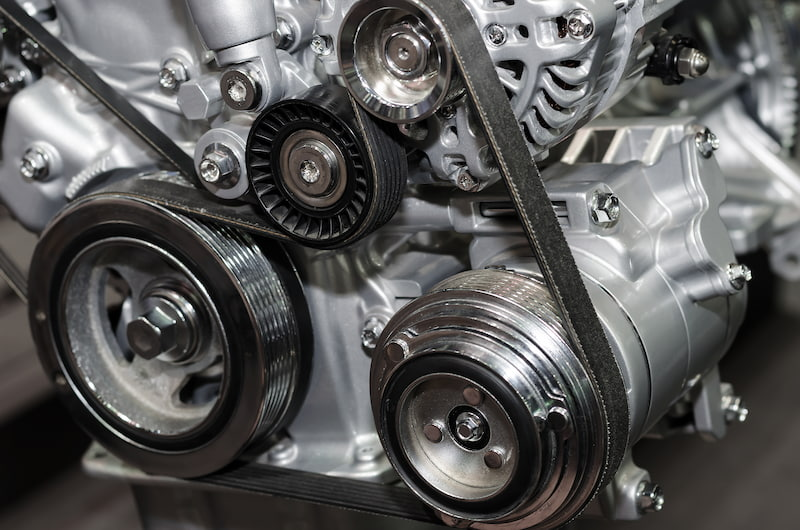
\includegraphics[scale=0.5]{Imagens/correia_carro.jpg}
	\fonte{\cite{correia_carro}}
\end{figure}


\chapter{Seleção de Correias Trapezoidais}


A seleção de correias se inicia com a definição dos parâmetros fundamentais do sistema de transmissão, sendo eles:

\begin{itemize}
    \item Potência a transmitir
    \item Rotação dos eixos
    \item Características do acionamento
    \item Estimativa de distância entre eixos
\end{itemize}

Pode-se dividir o processo de escolha em alguns passos bem definidos:

\section{Passo 01 - Definição da potência de projeto}

Com base na potência nominal, pode-se estimar a potência efetiva, com base nas condições de serviço, representadas por ${K_0}$.

\begin{equation}
    P_P=K_0\cdot N_0 \label{9.24}
\end{equation}

Os valores para ${K_0}$ são obtidos a partir da seguinte tabela:

\begin{figure}[h]
	\centering
	\caption{Fator de Serviço}
    \label{k0_tabela}
	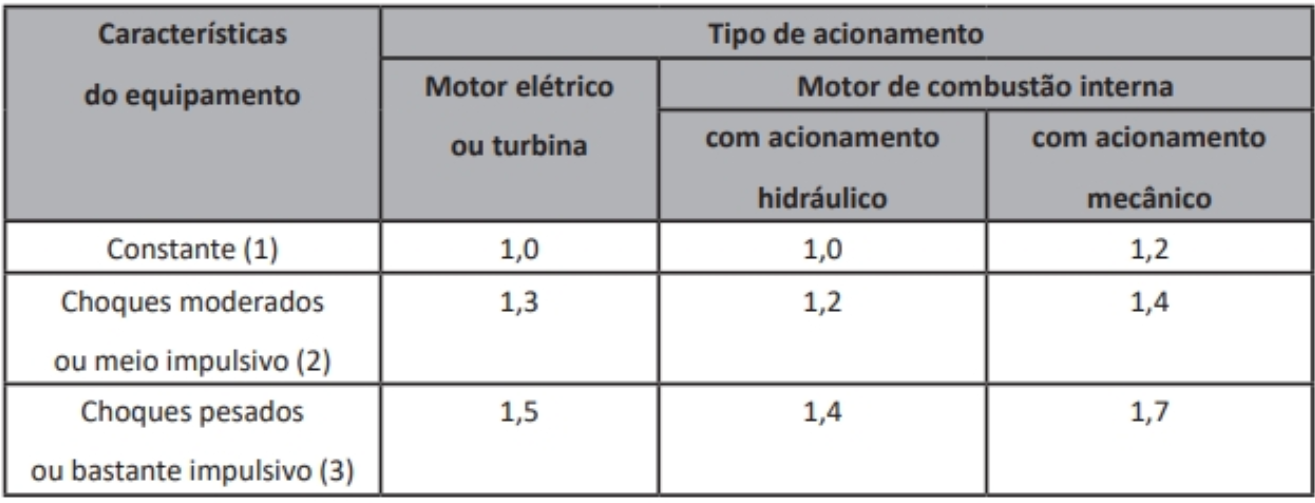
\includegraphics[scale=0.4]{Imagens/K0.png}
	\fonte{\cite{EMA_Barbieri}}
\end{figure}

\newpage
\section{Passo 02 - Definição do perfil da Correia}

Com base na potência e na rotação do eixo, pode-se utilizar a Figura~\ref{graf_perfis} para definir o perfil da correia

\begin{figure}[h]
	\centering
	\caption{Gráfico de seleção para correias trapezoidais.}
    \label{graf_perfis}
	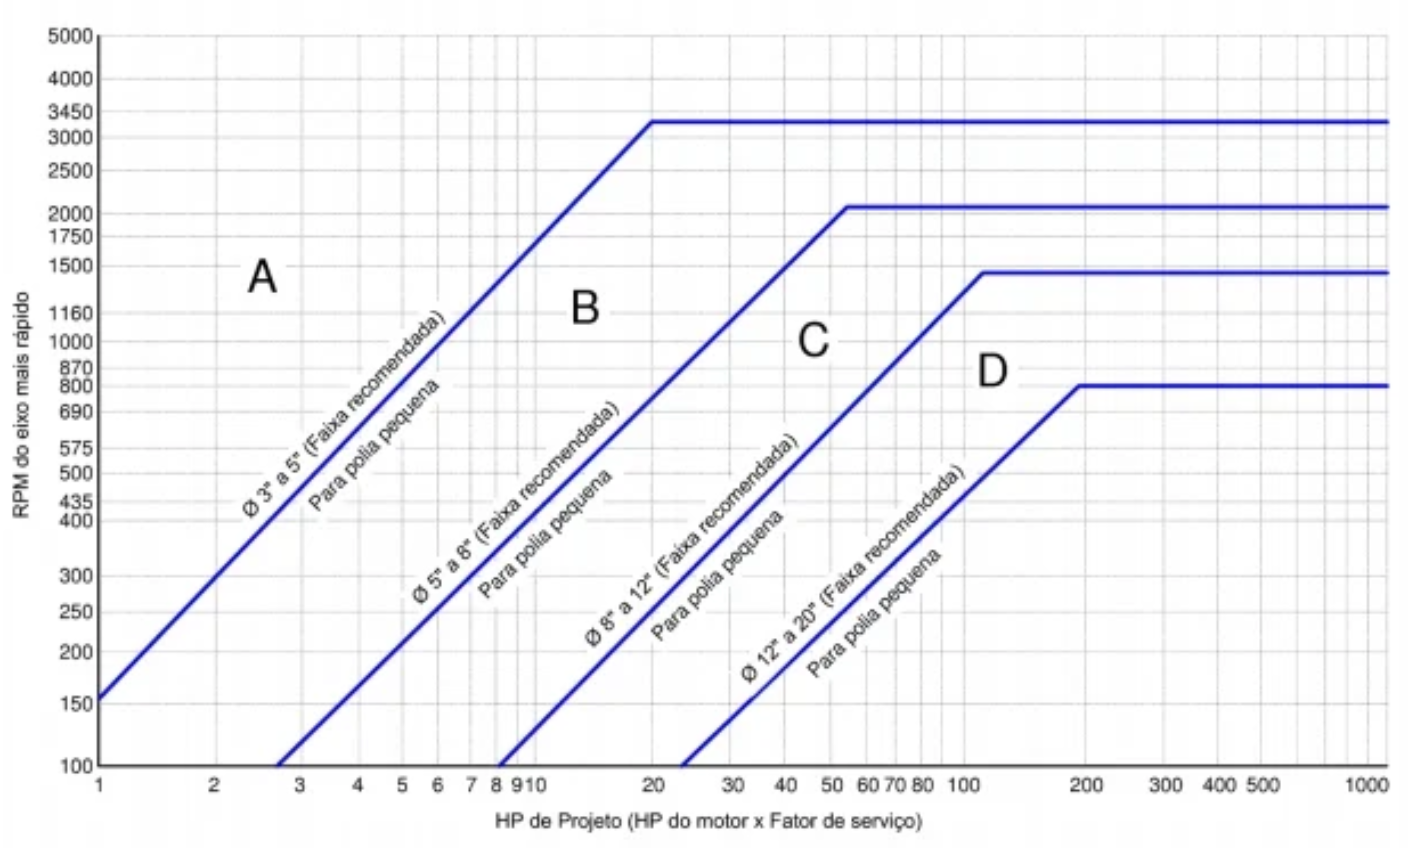
\includegraphics[scale=0.42]{Imagens/graf_perfis.png}
	\fonte{\cite{EMA_Barbieri}}
\end{figure}

\begin{figure}[h]
	\centering
	\caption{Opções de perfis de Correia}
    \label{perfis_correia}
	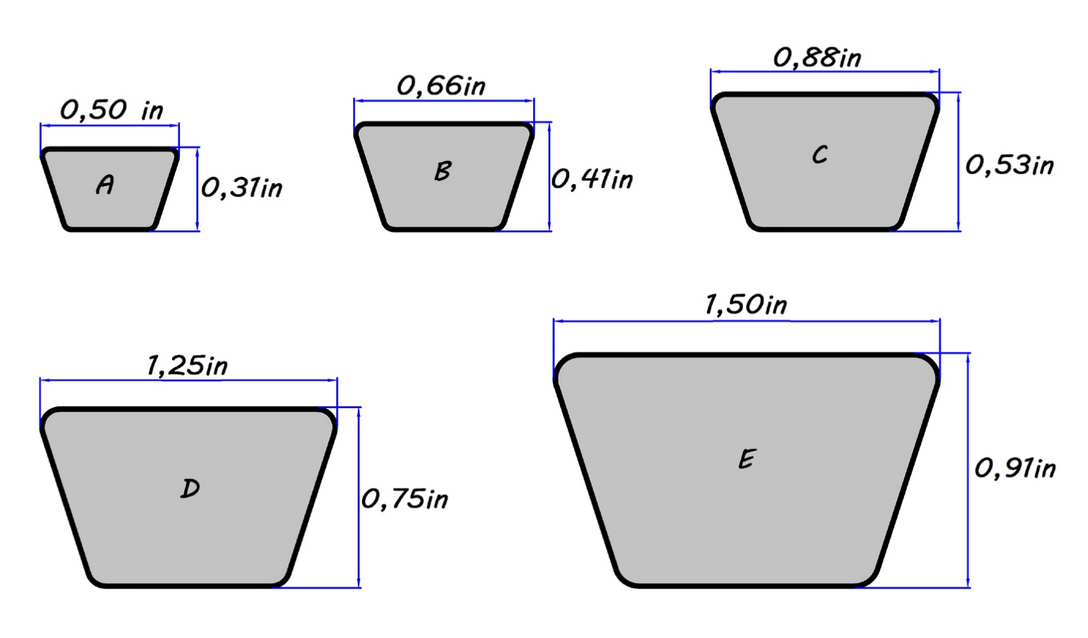
\includegraphics[scale=0.45]{Imagens/perfis_correia.png}
	\fonte{\cite{EMA_Barbieri}}
\end{figure}

\section{Passo 03 - Definição dos diâmetros das Polias}

Caso não haja definição do diâmetro da polia motora, deve-se adotar o diâmetro recomendado pela Figura~\ref{graf_perfis}. A polia movida é determinada a partir da razão de transmissão necessária.

\section{Passo 04 - Definição da velocidade tangencial da correia}

Possuindo todos os dados do sistema, pode-se calcular a velocidade da correia utilizando a Eq.~\eqref{v_correia}.

\begin{equation}
    v=w \cdot r_p=\frac{\pi \cdot d_p \cdot n}{60} \label{v_correia}
\end{equation}

Em termos práticos, a velocidade a correia não deve ultrapassar 20 m/s.

\section{Passo 05 - Definição do comprimento da correia e do ângulo de abraçamento da polia}

Com a definição dos diâmetros das polias e a distância entre centros pode-se calcular o comprimento da polia:

Abertas:
\begin{equation}
    L=2a + 1,57(dp_2+dp_1)+ \frac{(dp_2-dp_1)^{2}}{4a} \label{comprimento_correia}
\end{equation}

\bigskip
Cruzadas:
\begin{equation}
    L=2a + 1,57(dp_2+dp_1)+ \frac{(dp_2+dp_1)^{2}}{4a}
\end{equation}

\bigskip
E também o ângulo de contato:

\begin{equation}
    \theta=\pi \pm 2arcsen \left( \frac{dp_2 - dp_1}{2a} \right)
\end{equation}



\section{Passo 06 - Definição do comprimento padronizado da correia e correção da distância entre centros}

O comprimento da correia deve ser aproximado em um comprimento comercial, encontrado na Tabela~9.13 de \cite{EMA_Barbieri}. A diferença entre o comprimento original e o padronizado será corrigida na distância entre centros com base na Eq. \eqref{deixo}.

\begin{equation}
    a_{conv}=a-\left(\frac{L-L_{tab}}{2}\right)     \label{deixo}
\end{equation}


\section{Passo 07 - Determinação dos fatores de correção}

A fim de acomodar propriamente as correias padronizadas, pequenos ajustes nos ângulos de contato e comprimento devem ser realizados, utilizando as Figuras~\ref{correcao_arco} e \ref{correcao_comprimento}


\begin{figure}[h]
	\centering
	\caption{Fator de Correção Arco}
    \label{correcao_arco}
	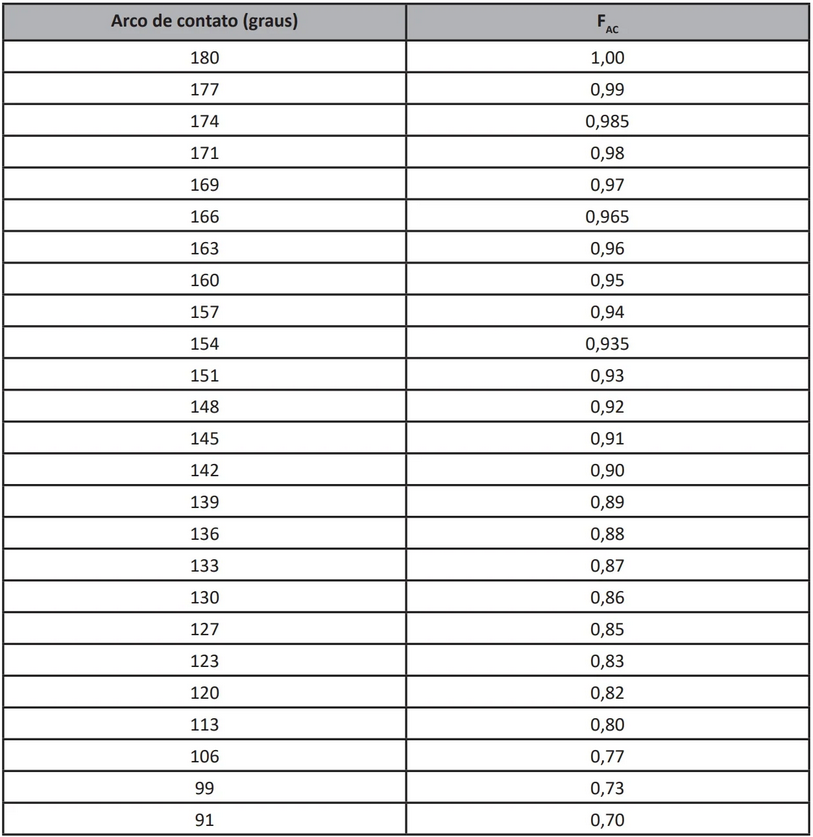
\includegraphics[scale=0.7]{Imagens/correcao_arco.png}
	\fonte{\cite{EMA_Barbieri}}
\end{figure}


\begin{figure}[p]
	\centering
	\caption{Fator de Correção Comprimento}
    \label{correcao_comprimento}
	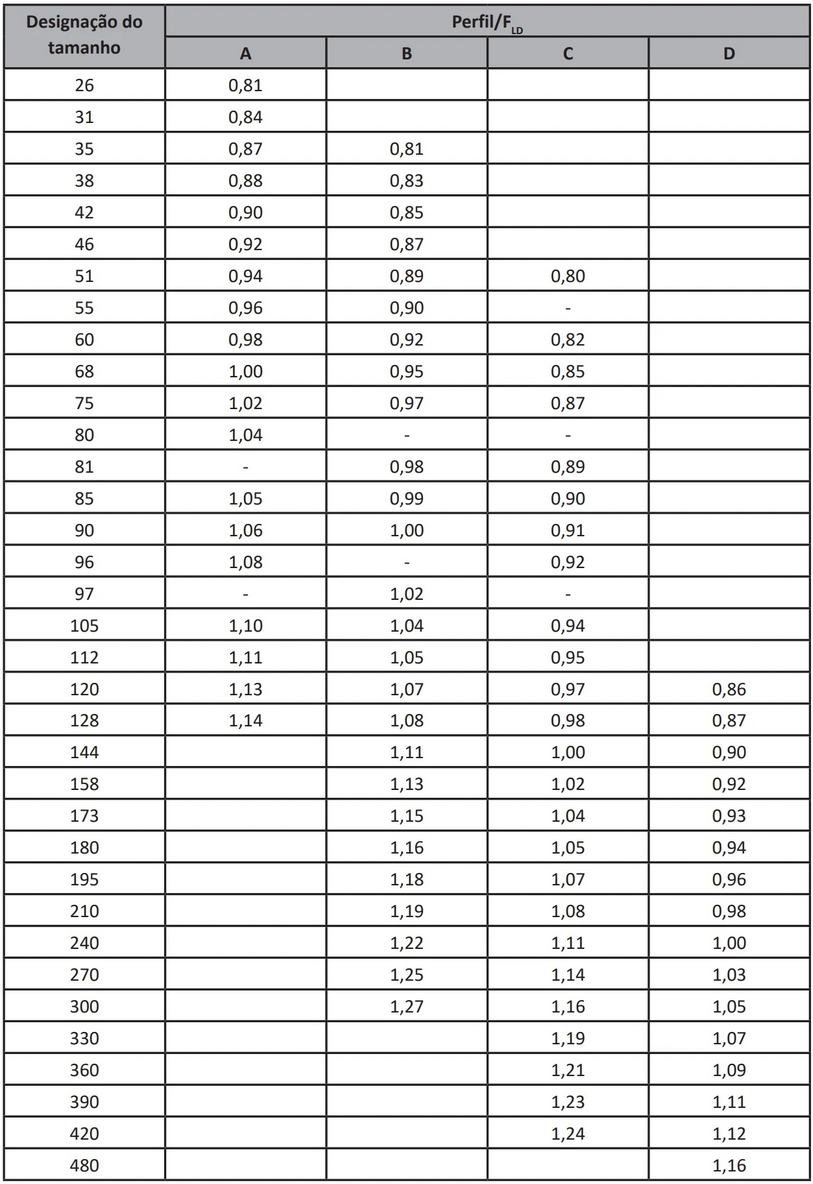
\includegraphics[scale=0.7]{Imagens/correcao_comprimento.png}
	\fonte{\cite{EMA_Barbieri}}
\end{figure}

\pagebreak
\section{Passo 08 - Determinação do HP básico e do HP adicional por correia}

Dada designação de correia possui parâmetros máximos de operação, utilizando as tabelas 9.6 a 9.9 e 9.6A a 9.9A de \cite{EMA_Barbieri}, pode-se estimar a potência básica e adicional

\begin{equation}
    HP_{class} = HP_{bas} + HP_{adic}
\end{equation}

\section{Passo 09 - Determinação do HP efetivo e do número de correias}

Com os fatores de correção em mãos, juntamente com os valores de potência, pode-se estimar a potência efetiva.
Também seno possível definir o número de correias necessárias para o projeto.


\begin{align}
    HP_{\text{efet}} &= HP_{\text{class}} \cdot F_{AC} \cdot F_{LP} \\
    N_{\text{correias}} &= \frac{P_p}{HP_{\text{efet}}}
\end{align}

\chapter{Seleção de Correias Sincronizadoras}

Para a escolha das polias sincronizadoras são necessários os parâmetros fundamentais para correias trapezoidais citados na seção 2.

\section{Passo 01 - Definição da potência do projeto}

Com base na Figura~\ref{k0_tabela} para se obter o fator de serviço, na Eq.\eqref{9.24} se consegue calcular a potência de projeto.


\section{Passo 02 - Definição da especificação da correia}

A partir da potência e da rotação do eixo motor, é possível determinar a especificação da correia utilizando a Figura~\ref{abaco_sinc}

\begin{figure}[h]
	\centering
	\caption{Ábaco seleção de correias sincronizadoras}
    \label{abaco_sinc}
	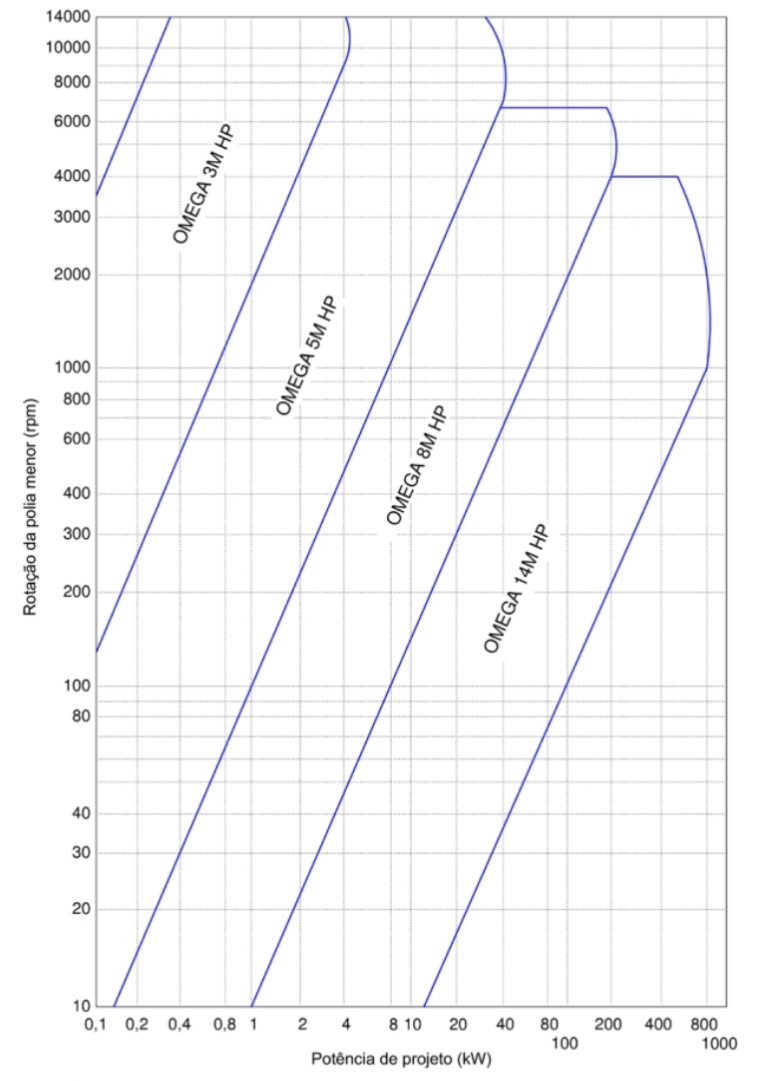
\includegraphics[scale=0.5]{Imagens/abaco_sinc.png}
	\fonte{\cite{EMA_Barbieri}}
\end{figure}

\section{Passo 03 - Definição dos números de dentes e diâmetros das polias}

Em função da potência de projeto e da rotação do eixo mais rápido, é possível definir o número de dentes mais recomendado para a polia motora, com base nas tabelas 9.10 a 9.13 de \cite{EMA_Barbieri}. Deve-se manter em mente o número mínimo de dentes recomendado para cada situação.

As tabelas de \cite{EMA_Barbieri} 9.20 a 9.23 fornecem o diâmetro das polias em função do número de dentes.

\section{Passo 04 - Definição da velocidade tangencial da correia}

Usa-se a Eq.~\eqref{v_correia} para determinar a velocidade tangencial da correia


\section{Passo 05 - Definição da distância entre eixos}

Para uma estimativa prévia da distância entre os eixos, pode-se usar as seguintes relações:

\begin{equation}
    a > 0,5(d_{p2} + d_{p1}) +15\text{mm} \qquad \text{e} \qquad a<2,0(d_{p2} + d_{p1})
\end{equation}

\section{Passo 06 - Cálculo do comprimento da correia}

Utiliza-se a Eq. \eqref{comprimento_correia} para o cálculo do comprimento da correia

\section{Passo 07 - Escolha do comprimento e correção da distância entre centros}

Efetiva-se os ajustes de comprimento com base nas Tabelas 9.14 a 9.17 de \cite{EMA_Barbieri}. O ajuste final é realizado usando a Eq. \eqref{deixo}.

\section{Passo 08 - Determinação de dentes em contato com a polia pequena}

É possível determinar a quantidade de dentes em contato com a polia pequena durante o funcionamento do sistema utilizando:

\begin{equation}
    z_e=\frac{z_1}{6} \left(3-\frac{d_{p2}-d_{p1}}{a_{corr}} \right)
\end{equation}



\section{Passo 09 - Determinação dos fatores de correção}

Como nas correias trapezoidais, fatores de correção precisam ser aplicados, são obtidos a partir das Figuras~\ref{correcao_dentes} e \ref{correcao_comp2}, com base no número de dentes em contato e o comprimento.

\begin{figure}[h]
	\centering
	\caption{Fator de correção com número de dentes}
    \label{correcao_dentes}
	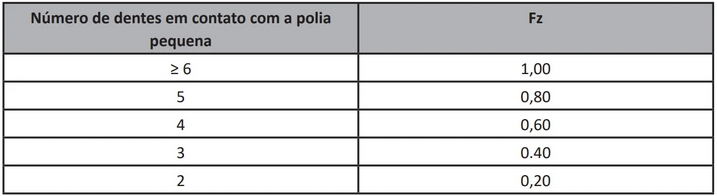
\includegraphics[scale=0.7]{Imagens/correcao_dentes.png}
	\fonte{\cite{EMA_Barbieri}}
\end{figure}

\begin{figure}[h]
	\centering
	\caption{Fator de correção com comprimento}
    \label{correcao_comp2}
	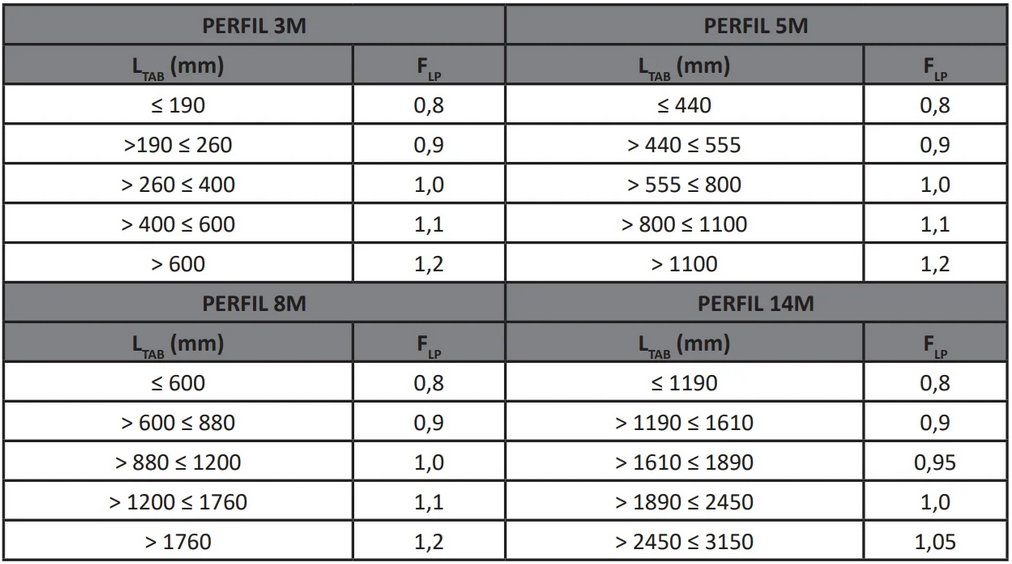
\includegraphics[scale=0.5]{Imagens/correcao_comp2.png}
	\fonte{\cite{EMA_Barbieri}}
\end{figure}

\pagebreak

\section{Passo 10 - Verificação da potência nominal da correia}

Os limites de potência nominal que as correias são capazes de transmitir estão presentes nas Tabelas 9.10 a 9.13 de \cite{EMA_Barbieri}, se encontram em função do número de dentes e da rotação. Deve-se verificar se a correia selecionada atende os requisitos do projeto, caso seja necessário deve-se selecionar uma largura de correia superior, a seguinte equação exibe essa relação.

\begin{equation}
    P_N F_{LP} F_Z \geq P_P
\end{equation}












% -----------------------------------------------------------------
% ELEMENTOS PÓS-TEXTUAIS
% -----------------------------------------------------------------
\postextual

% Você pode comentar os elementos que não deseja em seu trabalho;

% Referências bibliográficas

%Notar que os autores continuam sendo transpostos em maiúsculas, como preconiza a ABNT NBR 6023:2002. 
%Se, no entanto, não desejar seguir esta regra,
%crie um novo arquivo .bst (por exemplo, novoestilo.bst)a partir do estilo
%usado (abntex2-cite-alf ou abntex2-cite-num) e retire todas as expressões
%"u" change.case$, lembrando-se de indicar o novo arquivo como estilo, por exemplo, 
%\bibliographystyle{novoestilo}, e colocar o arquivo criado na mesma
%pasta em que está compilando o documento.

% Arquivo alterado para citação (Autor, Ano) ao invés de (AUTOR, Ano) conforme ABNT NBR 10520:2023
\bibliographystyle{abntex2-alf_revNBR2023.bst}	

\bibliography{abntex2-ref_UDESC_2020}	% Elemento Obrigatório

% % ----------------------------------------------------------
% Glossário
% ----------------------------------------------------------

%Consulte o manual da classe abntex2 para orientações sobre o glossário.

%\glossary




% ----------------------------------------------------------
% Glossário (Formatado Manualmente)
% ----------------------------------------------------------

\chapter*{GLOSSÁRIO}
\addcontentsline{toc}{chapter}{GLOSSÁRIO}

{ \setlength{\parindent}{0pt} % ambiente sem indentação

\textbf{Ardósia}: Rocha metamórfica sílico-argilosa formada pela transformação da argila sob pressão e temperatura, endurecida em finas lamelas.

\textbf{Arenito}: rocha sedimentária de origem detrítica formada de grãos agregados por um cimento natural silicoso, calcário ou ferruginoso que comunica ao conjunto em geral qualidades de dureza e compactação.

\textbf{Feldspato}: grupo de silicatos de sódio, potássio, cálcio ou outros elementos que compreende dois subgrupos, os feldspatos alcalinos e os plagioclásios.






} % fim ambiente sem indentação


				% Elemento Opcional
% 
% ----------------------------------------------------------
% Apêndices
% ----------------------------------------------------------

% ---
% Inicia os apêndices
% ---
\begin{apendicesenv}

% Imprime uma página indicando o início dos apêndices
%\partapendices

% ----------------------------------------------------------
\chapter{TÍTULO}
% ----------------------------------------------------------


\end{apendicesenv}
% ---				% Elemento Opcional
% 
% ----------------------------------------------------------
% Anexos
% ----------------------------------------------------------
%
% ---
% Inicia os anexos
% ---
\begin{anexosenv}

% Imprime uma página indicando o início dos anexos
%\partanexos

% ---
\chapter{TÍTULO}
% ---



\end{anexosenv}
				% Elemento Opcional
% 
%%---------------------------------------------------------------------
%% INDICE REMISSIVO
%%---------------------------------------------------------------------

%\phantompart
%\printindex

%---------------------------------------------------------------------

%%---------------------------------------------------------------------
%% INDICE REMISSIVO (Formatado Manualmente)
%%---------------------------------------------------------------------

\chapter*{ÍNDICE}
\addcontentsline{toc}{chapter}{ÍNDICE}

{ \setlength{\parindent}{0pt}  % ambiente sem indentação
	
Andesito, 22, 50, 73

Argila, 52, 75, 121

Basalto, 25, 230, 235

	
	
	
	
} % fim ambiente sem indentação


		% Elemento Opcional



\end{document}

% -----------------------------------------------------------------
% Fim do Documento
% -----------------------------------------------------------------	